\documentclass[tikz, border=14pt]{standalone}
\usepackage{tikz}
\usepackage{mathtools}
\usetikzlibrary{bayesnet}
\begin{document}
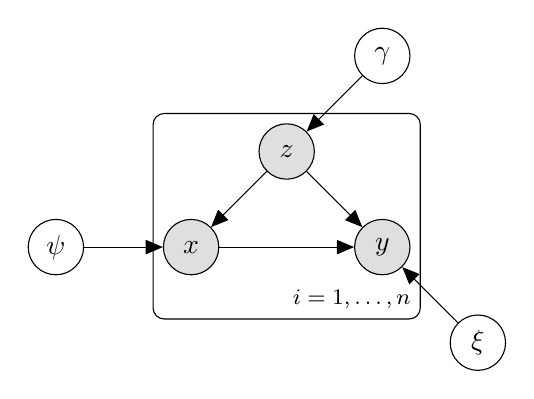
\begin{tikzpicture}
    \node[obs] (x) {$x$};
    \node[obs, above right = of x] (z) {$z$};
    \node[obs, below right = of z] (y) {$y$};
    \edge{x}{y};
    \edge{z}{y};
    \edge{z}{x};
    \plate {plate1} {(x)(y)(z)} {$i=1,\ldots, n$ };
        
    \node[latent, left = of x] (psi) {$\psi$}; 
    \node[latent, above right = of z] (gamma) {$\gamma$};
    \node[latent, below right = of y] (xi) {$\xi$};
    \edge{xi}{y};
    \edge{gamma}{z};
    \edge{psi}{x};
\end{tikzpicture}
\end{document}